\documentclass[twoside]{book}

% Packages required by doxygen
\usepackage{calc}
\usepackage{doxygen}
\usepackage{graphicx}
\usepackage[utf8]{inputenc}
\usepackage{makeidx}
\usepackage{multicol}
\usepackage{multirow}
\usepackage{textcomp}
\usepackage[table]{xcolor}

% Font selection
\usepackage[T1]{fontenc}
\usepackage{mathptmx}
\usepackage[scaled=.90]{helvet}
\usepackage{courier}
\usepackage{amssymb}
\usepackage{sectsty}
\renewcommand{\familydefault}{\sfdefault}
\allsectionsfont{%
  \fontseries{bc}\selectfont%
  \color{darkgray}%
}
\renewcommand{\DoxyLabelFont}{%
  \fontseries{bc}\selectfont%
  \color{darkgray}%
}

% Page & text layout
\usepackage{geometry}
\geometry{%
  a4paper,%
  top=2.5cm,%
  bottom=2.5cm,%
  left=2.5cm,%
  right=2.5cm%
}
\tolerance=750
\hfuzz=15pt
\hbadness=750
\setlength{\emergencystretch}{15pt}
\setlength{\parindent}{0cm}
\setlength{\parskip}{0.2cm}
\makeatletter
\renewcommand{\paragraph}{%
  \@startsection{paragraph}{4}{0ex}{-1.0ex}{1.0ex}{%
    \normalfont\normalsize\bfseries\SS@parafont%
  }%
}
\renewcommand{\subparagraph}{%
  \@startsection{subparagraph}{5}{0ex}{-1.0ex}{1.0ex}{%
    \normalfont\normalsize\bfseries\SS@subparafont%
  }%
}
\makeatother

% Headers & footers
\usepackage{fancyhdr}
\pagestyle{fancyplain}
\fancyhead[LE]{\fancyplain{}{\bfseries\thepage}}
\fancyhead[CE]{\fancyplain{}{}}
\fancyhead[RE]{\fancyplain{}{\bfseries\leftmark}}
\fancyhead[LO]{\fancyplain{}{\bfseries\rightmark}}
\fancyhead[CO]{\fancyplain{}{}}
\fancyhead[RO]{\fancyplain{}{\bfseries\thepage}}
\fancyfoot[LE]{\fancyplain{}{}}
\fancyfoot[CE]{\fancyplain{}{}}
\fancyfoot[RE]{\fancyplain{}{\bfseries\scriptsize Generated on Wed Jul 19 2017 16\-:00\-:26 for T\-Ue\-Lane\-Tracker by Doxygen }}
\fancyfoot[LO]{\fancyplain{}{\bfseries\scriptsize Generated on Wed Jul 19 2017 16\-:00\-:26 for T\-Ue\-Lane\-Tracker by Doxygen }}
\fancyfoot[CO]{\fancyplain{}{}}
\fancyfoot[RO]{\fancyplain{}{}}
\renewcommand{\footrulewidth}{0.4pt}
\renewcommand{\chaptermark}[1]{%
  \markboth{#1}{}%
}
\renewcommand{\sectionmark}[1]{%
  \markright{\thesection\ #1}%
}

% Indices & bibliography
\usepackage{natbib}
\usepackage[titles]{tocloft}
\setcounter{tocdepth}{3}
\setcounter{secnumdepth}{5}
\makeindex

% Hyperlinks (required, but should be loaded last)
\usepackage{ifpdf}
\ifpdf
  \usepackage[pdftex,pagebackref=true]{hyperref}
\else
  \usepackage[ps2pdf,pagebackref=true]{hyperref}
\fi
\hypersetup{%
  colorlinks=true,%
  linkcolor=blue,%
  citecolor=blue,%
  unicode%
}

% Custom commands
\newcommand{\clearemptydoublepage}{%
  \newpage{\pagestyle{empty}\cleardoublepage}%
}


%===== C O N T E N T S =====

\begin{document}

% Titlepage & ToC
\hypersetup{pageanchor=false}
\pagenumbering{roman}
\begin{titlepage}
\vspace*{7cm}
\begin{center}%
{\Large T\-Ue\-Lane\-Tracker }\\
\vspace*{1cm}
{\large Generated by Doxygen 1.8.6}\\
\vspace*{0.5cm}
{\small Wed Jul 19 2017 16:00:26}\\
\end{center}
\end{titlepage}
\clearemptydoublepage
\tableofcontents
\clearemptydoublepage
\pagenumbering{arabic}
\hypersetup{pageanchor=true}

%--- Begin generated contents ---
\chapter{Welcome to T\-Ue\-Lane Tracker}
\label{index}\hypertarget{index}{}\begin{DoxyAuthor}{Author}
Rameez Ismail
\end{DoxyAuthor}
This is a software application that detects and tracks lanes on the road. The underlying algorithm is a probabilistic algorithm which is originally developed at, under the strategic area of Smart Mobility, Eindhoven University of Technology (T\-U/e). The algorithm exploits the concept of hierarchical classification from deep learning however, unlike deep learning, classification at each hierarchical level is engineered instead of being trained through images. This make it more predictable as well as verifiable. The software application is completely object oriented and follows various software design principles recommended by safety standard I\-S\-O26262.

This application provide a loose coupling between the software control flow and actual realisation of the algorithm, making it possible to generate various target specific implementations of the algorithm. Current version of the software applicataion is developed in cooperation with N\-X\-P Semiconductors. This repository provides real-\/time generic implementation of the algorithm using Open\-C\-V library. A real time embedded implementation, using N\-X\-P Bluebox, is underdevelopment.\hypertarget{index_Purpose}{}\section{Purpose}\label{index_Purpose}
\hypertarget{index_Architecture}{}\section{Application Architecture}\label{index_Architecture}
The software application architecture is explained using following views
\begin{DoxyItemize}
\item \hyperlink{static}{Static View}
\item \hyperlink{process}{Process View}
\item Development View
\end{DoxyItemize}\hypertarget{index_installing}{}\section{Appliction Installation}\label{index_installing}
\hypertarget{index_running}{}\section{Running the Application}\label{index_running}

\chapter{Hierarchical Index}
\section{Class Hierarchy}
This inheritance list is sorted roughly, but not completely, alphabetically\-:\begin{DoxyCompactList}
\item \contentsline{section}{Base\-Histogram\-Model}{\pageref{structBaseHistogramModel}}{}
\item \contentsline{section}{Buffering\-D\-A\-G\-\_\-generic}{\pageref{classBufferingDAG__generic}}{}
\begin{DoxyCompactList}
\item \contentsline{section}{Tracking\-Lane\-D\-A\-G\-\_\-generic}{\pageref{classTrackingLaneDAG__generic}}{}
\end{DoxyCompactList}
\item \contentsline{section}{Buffer\-Pool}{\pageref{structBufferPool}}{}
\item \contentsline{section}{Camera}{\pageref{structCamera}}{}
\item \contentsline{section}{Car}{\pageref{structCar}}{}
\item \contentsline{section}{Lane\-Filter}{\pageref{classLaneFilter}}{}
\item \contentsline{section}{Lane\-Membership}{\pageref{structLaneMembership}}{}
\item \contentsline{section}{Lane\-Model}{\pageref{structLaneModel}}{}
\item \contentsline{section}{Lane\-Parameters}{\pageref{structLaneParameters}}{}
\item \contentsline{section}{Purview\-Histogram\-Model}{\pageref{structPurviewHistogramModel}}{}
\item \contentsline{section}{State}{\pageref{classState}}{}
\begin{DoxyCompactList}
\item \contentsline{section}{Buffering\-State}{\pageref{classBufferingState}}{}
\item \contentsline{section}{Init\-State}{\pageref{classInitState}}{}
\item \contentsline{section}{Tracking\-Lane\-State}{\pageref{classTrackingLaneState}}{}
\end{DoxyCompactList}
\item \contentsline{section}{State\-Machine}{\pageref{classStateMachine}}{}
\item \contentsline{section}{Templates}{\pageref{structTemplates}}{}
\item \contentsline{section}{Vanishing\-Pt}{\pageref{structVanishingPt}}{}
\item \contentsline{section}{Vanishing\-Pt\-Filter}{\pageref{classVanishingPtFilter}}{}
\end{DoxyCompactList}

\chapter{Class Index}
\section{Class List}
Here are the classes, structs, unions and interfaces with brief descriptions\-:\begin{DoxyCompactList}
\item\contentsline{section}{\hyperlink{structBaseHistogramModel}{Base\-Histogram\-Model} }{\pageref{structBaseHistogramModel}}{}
\item\contentsline{section}{\hyperlink{classBufferingDAG__generic}{Buffering\-D\-A\-G\-\_\-generic} }{\pageref{classBufferingDAG__generic}}{}
\item\contentsline{section}{\hyperlink{classBufferingState}{Buffering\-State} }{\pageref{classBufferingState}}{}
\item\contentsline{section}{\hyperlink{structBufferPool}{Buffer\-Pool} }{\pageref{structBufferPool}}{}
\item\contentsline{section}{\hyperlink{structCamera}{Camera} }{\pageref{structCamera}}{}
\item\contentsline{section}{\hyperlink{structCar}{Car} }{\pageref{structCar}}{}
\item\contentsline{section}{\hyperlink{classInitState}{Init\-State} }{\pageref{classInitState}}{}
\item\contentsline{section}{\hyperlink{classLaneFilter}{Lane\-Filter} }{\pageref{classLaneFilter}}{}
\item\contentsline{section}{\hyperlink{structLaneMembership}{Lane\-Membership} }{\pageref{structLaneMembership}}{}
\item\contentsline{section}{\hyperlink{structLaneModel}{Lane\-Model} }{\pageref{structLaneModel}}{}
\item\contentsline{section}{\hyperlink{structLaneParameters}{Lane\-Parameters} }{\pageref{structLaneParameters}}{}
\item\contentsline{section}{\hyperlink{structPurviewHistogramModel}{Purview\-Histogram\-Model} }{\pageref{structPurviewHistogramModel}}{}
\item\contentsline{section}{\hyperlink{classState}{State} }{\pageref{classState}}{}
\item\contentsline{section}{\hyperlink{classStateMachine}{State\-Machine} }{\pageref{classStateMachine}}{}
\item\contentsline{section}{\hyperlink{structTemplates}{Templates} }{\pageref{structTemplates}}{}
\item\contentsline{section}{\hyperlink{classTrackingLaneDAG__generic}{Tracking\-Lane\-D\-A\-G\-\_\-generic} }{\pageref{classTrackingLaneDAG__generic}}{}
\item\contentsline{section}{\hyperlink{classTrackingLaneState}{Tracking\-Lane\-State} }{\pageref{classTrackingLaneState}}{}
\item\contentsline{section}{\hyperlink{structVanishingPt}{Vanishing\-Pt} }{\pageref{structVanishingPt}}{}
\item\contentsline{section}{\hyperlink{classVanishingPtFilter}{Vanishing\-Pt\-Filter} }{\pageref{classVanishingPtFilter}}{}
\end{DoxyCompactList}

\chapter{File Index}
\section{File List}
Here is a list of all documented files with brief descriptions\-:\begin{DoxyCompactList}
\item\contentsline{section}{/home/rameez/\-Master/\-T\-Ue\-Lane\-Tracker/\-Lane\-Tracker\-App/\hyperlink{main_8cpp}{main.\-cpp} }{\pageref{main_8cpp}}{}
\item\contentsline{section}{/home/rameez/\-Master/\-T\-Ue\-Lane\-Tracker/\-Lane\-Tracker\-App/include/{\bfseries Main\-Page.\-h} }{\pageref{MainPage_8h}}{}
\item\contentsline{section}{/home/rameez/\-Master/\-T\-Ue\-Lane\-Tracker/\-T\-Ue\-L\-D\-T/include/{\bfseries Buffering\-D\-A\-G\-\_\-generic.\-h} }{\pageref{BufferingDAG__generic_8h}}{}
\item\contentsline{section}{/home/rameez/\-Master/\-T\-Ue\-Lane\-Tracker/\-T\-Ue\-L\-D\-T/include/{\bfseries Buffering\-State.\-h} }{\pageref{BufferingState_8h}}{}
\item\contentsline{section}{/home/rameez/\-Master/\-T\-Ue\-Lane\-Tracker/\-T\-Ue\-L\-D\-T/include/{\bfseries Camera.\-h} }{\pageref{Camera_8h}}{}
\item\contentsline{section}{/home/rameez/\-Master/\-T\-Ue\-Lane\-Tracker/\-T\-Ue\-L\-D\-T/include/{\bfseries Car.\-h} }{\pageref{Car_8h}}{}
\item\contentsline{section}{/home/rameez/\-Master/\-T\-Ue\-Lane\-Tracker/\-T\-Ue\-L\-D\-T/include/{\bfseries Init\-State.\-h} }{\pageref{InitState_8h}}{}
\item\contentsline{section}{/home/rameez/\-Master/\-T\-Ue\-Lane\-Tracker/\-T\-Ue\-L\-D\-T/include/{\bfseries Lane.\-h} }{\pageref{Lane_8h}}{}
\item\contentsline{section}{/home/rameez/\-Master/\-T\-Ue\-Lane\-Tracker/\-T\-Ue\-L\-D\-T/include/{\bfseries Lane\-Filter.\-h} }{\pageref{LaneFilter_8h}}{}
\item\contentsline{section}{/home/rameez/\-Master/\-T\-Ue\-Lane\-Tracker/\-T\-Ue\-L\-D\-T/include/{\bfseries Scaling\-Factors.\-h} }{\pageref{ScalingFactors_8h}}{}
\item\contentsline{section}{/home/rameez/\-Master/\-T\-Ue\-Lane\-Tracker/\-T\-Ue\-L\-D\-T/include/{\bfseries State.\-h} }{\pageref{State_8h}}{}
\item\contentsline{section}{/home/rameez/\-Master/\-T\-Ue\-Lane\-Tracker/\-T\-Ue\-L\-D\-T/include/{\bfseries State\-Machine.\-h} }{\pageref{StateMachine_8h}}{}
\item\contentsline{section}{/home/rameez/\-Master/\-T\-Ue\-Lane\-Tracker/\-T\-Ue\-L\-D\-T/include/{\bfseries Templates.\-h} }{\pageref{Templates_8h}}{}
\item\contentsline{section}{/home/rameez/\-Master/\-T\-Ue\-Lane\-Tracker/\-T\-Ue\-L\-D\-T/include/{\bfseries Tracking\-Lane\-D\-A\-G\-\_\-generic.\-h} }{\pageref{TrackingLaneDAG__generic_8h}}{}
\item\contentsline{section}{/home/rameez/\-Master/\-T\-Ue\-Lane\-Tracker/\-T\-Ue\-L\-D\-T/include/{\bfseries Tracking\-Lane\-State.\-h} }{\pageref{TrackingLaneState_8h}}{}
\item\contentsline{section}{/home/rameez/\-Master/\-T\-Ue\-Lane\-Tracker/\-T\-Ue\-L\-D\-T/include/{\bfseries Vanishing\-Pt\-Filter.\-h} }{\pageref{VanishingPtFilter_8h}}{}
\end{DoxyCompactList}

\chapter{Class Documentation}
\hypertarget{structBaseHistogramModel}{\section{Base\-Histogram\-Model Struct Reference}
\label{structBaseHistogramModel}\index{Base\-Histogram\-Model@{Base\-Histogram\-Model}}
}
\subsection*{Public Attributes}
\begin{DoxyCompactItemize}
\item 
\hypertarget{structBaseHistogramModel_ae129cc9360fe03bc507b9fc89f455025}{int {\bfseries left\-Offset\-Idx}}\label{structBaseHistogramModel_ae129cc9360fe03bc507b9fc89f455025}

\item 
\hypertarget{structBaseHistogramModel_abbcbeba514302e037328fde2f60ea068}{int {\bfseries right\-Offset\-Idx}}\label{structBaseHistogramModel_abbcbeba514302e037328fde2f60ea068}

\item 
\hypertarget{structBaseHistogramModel_ab6e7d8809d74a9fa63b182e695727738}{int {\bfseries left\-Offset}}\label{structBaseHistogramModel_ab6e7d8809d74a9fa63b182e695727738}

\item 
\hypertarget{structBaseHistogramModel_a72b2b16eed857713bd39d38d02d8b79f}{int {\bfseries right\-Offset}}\label{structBaseHistogramModel_a72b2b16eed857713bd39d38d02d8b79f}

\item 
\hypertarget{structBaseHistogramModel_a1da0e4b89eeeb6185fdb31ba6e5af0f3}{float {\bfseries width\-\_\-cm}}\label{structBaseHistogramModel_a1da0e4b89eeeb6185fdb31ba6e5af0f3}

\item 
\hypertarget{structBaseHistogramModel_a99cfaa485a8c836e196cf4b36d30c913}{int {\bfseries bin\-I\-D\-\_\-left\-Boundary}}\label{structBaseHistogramModel_a99cfaa485a8c836e196cf4b36d30c913}

\item 
\hypertarget{structBaseHistogramModel_abb73c06cd993b879c00c5a8351516f43}{int {\bfseries bin\-I\-D\-\_\-right\-Boundary}}\label{structBaseHistogramModel_abb73c06cd993b879c00c5a8351516f43}

\item 
\hypertarget{structBaseHistogramModel_a0bea845eaa4a3449c5a0b5fff53cf1c7}{int {\bfseries bin\-I\-D\-\_\-\-Neg\-Boundary\-Left}}\label{structBaseHistogramModel_a0bea845eaa4a3449c5a0b5fff53cf1c7}

\item 
\hypertarget{structBaseHistogramModel_a3b74b913158fec0ba82298d40b30b238}{int {\bfseries nb\-Non\-Boundary\-Bins\-Left}}\label{structBaseHistogramModel_a3b74b913158fec0ba82298d40b30b238}

\item 
\hypertarget{structBaseHistogramModel_adf103bbe2f65b82dbfa0f5fe3301031a}{int {\bfseries bin\-I\-D\-\_\-\-Neg\-Boundary\-Right}}\label{structBaseHistogramModel_adf103bbe2f65b82dbfa0f5fe3301031a}

\item 
\hypertarget{structBaseHistogramModel_af19b255aae30a4762453fcbeab0c5128}{int {\bfseries nb\-Non\-Boundary\-Bins\-Right}}\label{structBaseHistogramModel_af19b255aae30a4762453fcbeab0c5128}

\end{DoxyCompactItemize}


The documentation for this struct was generated from the following file\-:\begin{DoxyCompactItemize}
\item 
/home/rameez/\-Master/\-T\-Ue\-Lane\-Tracker/\-T\-Ue\-L\-D\-T/include/Lane\-Filter.\-h\end{DoxyCompactItemize}

\hypertarget{classBufferingDAG__generic}{\section{Buffering\-D\-A\-G\-\_\-generic Class Reference}
\label{classBufferingDAG__generic}\index{Buffering\-D\-A\-G\-\_\-generic@{Buffering\-D\-A\-G\-\_\-generic}}
}
Inheritance diagram for Buffering\-D\-A\-G\-\_\-generic\-:\begin{figure}[H]
\begin{center}
\leavevmode
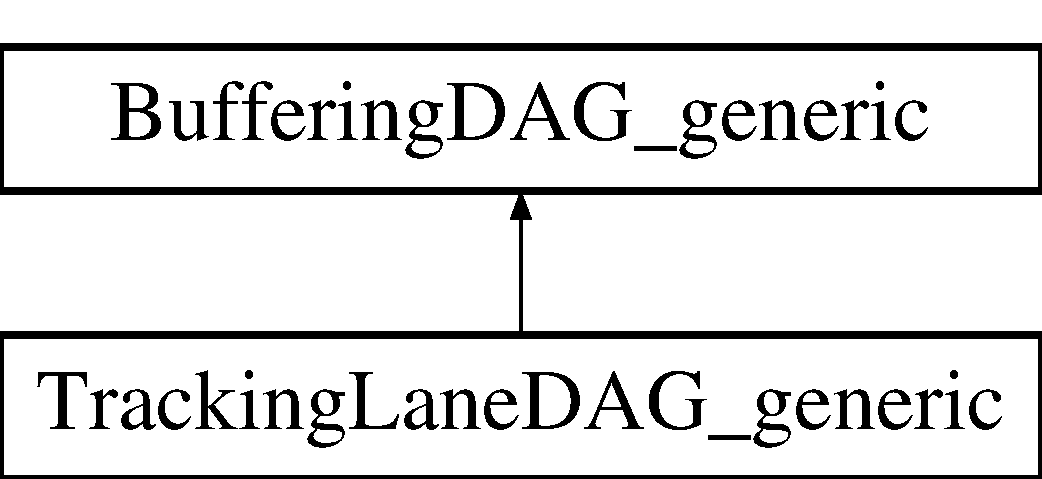
\includegraphics[height=2.000000cm]{classBufferingDAG__generic}
\end{center}
\end{figure}
\subsection*{Public Member Functions}
\begin{DoxyCompactItemize}
\item 
\hypertarget{classBufferingDAG__generic_a0e1ee4f8a694fd0fdf2b9893944929e8}{int {\bfseries grab\-Frame} ()}\label{classBufferingDAG__generic_a0e1ee4f8a694fd0fdf2b9893944929e8}

\item 
\hypertarget{classBufferingDAG__generic_a7d58d28db3981dac7aaed4b1badb5d88}{void {\bfseries auxillary\-Tasks} ()}\label{classBufferingDAG__generic_a7d58d28db3981dac7aaed4b1badb5d88}

\item 
\hypertarget{classBufferingDAG__generic_a34a33f6c25ab56c002bb4cd67a9c990c}{void {\bfseries buffer} ()}\label{classBufferingDAG__generic_a34a33f6c25ab56c002bb4cd67a9c990c}

\item 
\hypertarget{classBufferingDAG__generic_a06d2690141f61dec3a1c55fb28d52d22}{{\bfseries Buffering\-D\-A\-G\-\_\-generic} (\hyperlink{classBufferingDAG__generic}{Buffering\-D\-A\-G\-\_\-generic} \&\&buffering\-Graph)}\label{classBufferingDAG__generic_a06d2690141f61dec3a1c55fb28d52d22}

\end{DoxyCompactItemize}
\subsection*{Protected Types}
\begin{DoxyCompactItemize}
\item 
\hypertarget{classBufferingDAG__generic_aee268cc775360e87f89fd05a72f21ec3}{using {\bfseries Mutex\-Type} = std\-::mutex}\label{classBufferingDAG__generic_aee268cc775360e87f89fd05a72f21ec3}

\item 
\hypertarget{classBufferingDAG__generic_af3b29cf93b8f1f13d4c2c5d369daf999}{using {\bfseries Write\-Lock} = std\-::unique\-\_\-lock$<$ Mutex\-Type $>$}\label{classBufferingDAG__generic_af3b29cf93b8f1f13d4c2c5d369daf999}

\end{DoxyCompactItemize}
\subsection*{Protected Attributes}
\begin{DoxyCompactItemize}
\item 
\hypertarget{classBufferingDAG__generic_af879ecf94770c873deaff67a9ad6025d}{Mutex\-Type {\bfseries \-\_\-mutex}}\label{classBufferingDAG__generic_af879ecf94770c873deaff67a9ad6025d}

\item 
\hypertarget{classBufferingDAG__generic_a6341f9fc09996792aa87904262ed1021}{condition\-\_\-variable {\bfseries \-\_\-sate\-Change}}\label{classBufferingDAG__generic_a6341f9fc09996792aa87904262ed1021}

\item 
\hypertarget{classBufferingDAG__generic_adc18bb042c1ecc8d7bc0b06eef486883}{bool {\bfseries m\-Buffer\-Ready} = false}\label{classBufferingDAG__generic_adc18bb042c1ecc8d7bc0b06eef486883}

\item 
\hypertarget{classBufferingDAG__generic_a2bdef2f9b832ee9be9ce191bbb45ecdd}{int {\bfseries m\-Span}}\label{classBufferingDAG__generic_a2bdef2f9b832ee9be9ce191bbb45ecdd}

\item 
\hypertarget{classBufferingDAG__generic_a544dea7677a3b16c844cc5abf8ba0a3f}{int {\bfseries m\-Margin}}\label{classBufferingDAG__generic_a544dea7677a3b16c844cc5abf8ba0a3f}

\item 
\hypertarget{classBufferingDAG__generic_a61137ddfd7dd16a776addb32212c6504}{int {\bfseries m\-V\-P\-\_\-\-Range\-\_\-\-V}}\label{classBufferingDAG__generic_a61137ddfd7dd16a776addb32212c6504}

\item 
\hypertarget{classBufferingDAG__generic_a637579defa89ce38045c17af56fe9c2c}{Mat {\bfseries m\-G\-R\-A\-D\-I\-E\-N\-T\-\_\-\-T\-A\-N\-\_\-\-R\-O\-O\-T}}\label{classBufferingDAG__generic_a637579defa89ce38045c17af56fe9c2c}

\item 
\hypertarget{classBufferingDAG__generic_a3405cbeb082d1e325619503bcfce78c8}{Mat {\bfseries m\-F\-O\-C\-U\-S\-\_\-\-M\-A\-S\-K\-\_\-\-R\-O\-O\-T}}\label{classBufferingDAG__generic_a3405cbeb082d1e325619503bcfce78c8}

\item 
\hypertarget{classBufferingDAG__generic_a7345dc24ebe8cb7e0eefb571cf40513f}{Mat {\bfseries m\-D\-E\-P\-T\-H\-\_\-\-M\-A\-P\-\_\-\-R\-O\-O\-T}}\label{classBufferingDAG__generic_a7345dc24ebe8cb7e0eefb571cf40513f}

\item 
\hypertarget{classBufferingDAG__generic_ab6676cc4a2b32f5386420794df2dc0cb}{unique\-\_\-ptr$<$ \hyperlink{structBufferPool}{Buffer\-Pool} $>$ {\bfseries m\-Buffer\-Pool}}\label{classBufferingDAG__generic_ab6676cc4a2b32f5386420794df2dc0cb}

\item 
\hypertarget{classBufferingDAG__generic_a3f5ecf31daf744fe63ee7a4218da4e2f}{const \hyperlink{structCamera}{Camera} {\bfseries m\-C\-A\-M\-E\-R\-A}}\label{classBufferingDAG__generic_a3f5ecf31daf744fe63ee7a4218da4e2f}

\item 
\hypertarget{classBufferingDAG__generic_aa91e170d5f81edaa18581cf9f5c81e43}{const \hyperlink{structLaneMembership}{Lane\-Membership} {\bfseries m\-Lane\-Membership}}\label{classBufferingDAG__generic_aa91e170d5f81edaa18581cf9f5c81e43}

\item 
\hypertarget{classBufferingDAG__generic_acce7fc93b09bbe166aba16d715a8cb26}{\hyperlink{structVanishingPt}{Vanishing\-Pt} {\bfseries m\-Vanish\-Pt}}\label{classBufferingDAG__generic_acce7fc93b09bbe166aba16d715a8cb26}

\item 
\hypertarget{classBufferingDAG__generic_a8033352cce24f0e9d96c49328f8180c2}{Mat {\bfseries m\-Frame\-R\-G\-B}}\label{classBufferingDAG__generic_a8033352cce24f0e9d96c49328f8180c2}

\item 
\hypertarget{classBufferingDAG__generic_a599ee714259c7a1b17f2c70f31020108}{Mat {\bfseries m\-Frame\-G\-R\-A\-Y}}\label{classBufferingDAG__generic_a599ee714259c7a1b17f2c70f31020108}

\item 
\hypertarget{classBufferingDAG__generic_a92c76720cf3d2a6dbd53eba2bdafcb03}{Mat {\bfseries m\-Frame\-G\-R\-A\-Y\-\_\-\-R\-O\-I}}\label{classBufferingDAG__generic_a92c76720cf3d2a6dbd53eba2bdafcb03}

\item 
\hypertarget{classBufferingDAG__generic_abaed06745e73e463d4fab4d9b98371e6}{Mat {\bfseries m\-Mask}}\label{classBufferingDAG__generic_abaed06745e73e463d4fab4d9b98371e6}

\item 
\hypertarget{classBufferingDAG__generic_a7ca79a2d779c55ea8497a9606996c7b9}{Mat {\bfseries m\-Grad\-X}}\label{classBufferingDAG__generic_a7ca79a2d779c55ea8497a9606996c7b9}

\item 
\hypertarget{classBufferingDAG__generic_ae08d118e71cafb27673c6b0049974e61}{Mat {\bfseries m\-Grad\-Y}}\label{classBufferingDAG__generic_ae08d118e71cafb27673c6b0049974e61}

\item 
\hypertarget{classBufferingDAG__generic_a18448e2e54c401207b24e4ccbf703f44}{Mat {\bfseries m\-Grad\-X\-\_\-abs}}\label{classBufferingDAG__generic_a18448e2e54c401207b24e4ccbf703f44}

\item 
\hypertarget{classBufferingDAG__generic_aa261d218e9d85dcf06d019677275f30e}{Mat {\bfseries m\-Grad\-Y\-\_\-abs}}\label{classBufferingDAG__generic_aa261d218e9d85dcf06d019677275f30e}

\item 
\hypertarget{classBufferingDAG__generic_af971e5dcf352f95ca402129ce2148edf}{Mat {\bfseries m\-Frame\-Grad\-Mag}}\label{classBufferingDAG__generic_af971e5dcf352f95ca402129ce2148edf}

\item 
\hypertarget{classBufferingDAG__generic_adcf79e354c59053c73f18a94f5f806a1}{Mat {\bfseries m\-Grad\-Tan\-Template}}\label{classBufferingDAG__generic_adcf79e354c59053c73f18a94f5f806a1}

\item 
\hypertarget{classBufferingDAG__generic_a5438b4439859e3668e02ee43b793ef33}{Mat {\bfseries m\-Depth\-Template}}\label{classBufferingDAG__generic_a5438b4439859e3668e02ee43b793ef33}

\item 
\hypertarget{classBufferingDAG__generic_a0d2c7b38fff3307f45242fe5808aca57}{Mat {\bfseries m\-Focus\-Template}}\label{classBufferingDAG__generic_a0d2c7b38fff3307f45242fe5808aca57}

\item 
\hypertarget{classBufferingDAG__generic_a95b8dbe5a220f1eede4cb021abb5a79b}{Mat {\bfseries m\-X\-\_\-\-V\-P\-R\-S}}\label{classBufferingDAG__generic_a95b8dbe5a220f1eede4cb021abb5a79b}

\item 
\hypertarget{classBufferingDAG__generic_aecd1a5bfd2cc730028f4c0e93549b5b2}{Mat {\bfseries m\-Y\-\_\-\-V\-P\-R\-S}}\label{classBufferingDAG__generic_aecd1a5bfd2cc730028f4c0e93549b5b2}

\item 
\hypertarget{classBufferingDAG__generic_ac8e573e248cf6c2ae5753295985f2e35}{Mat {\bfseries m\-Temp\-Prob\-Mat}}\label{classBufferingDAG__generic_ac8e573e248cf6c2ae5753295985f2e35}

\item 
\hypertarget{classBufferingDAG__generic_ac655ff8f94e89cc25b7597dfe893e4db}{Mat {\bfseries m\-Prob\-Map\-\_\-\-Gray}}\label{classBufferingDAG__generic_ac655ff8f94e89cc25b7597dfe893e4db}

\item 
\hypertarget{classBufferingDAG__generic_a700212b57de614f4763d8b345c2a06c4}{Mat {\bfseries m\-Prob\-Map\-\_\-\-Grad\-Mag}}\label{classBufferingDAG__generic_a700212b57de614f4763d8b345c2a06c4}

\item 
\hypertarget{classBufferingDAG__generic_a10a2b2efa34a2908ca713a81a0ebceed}{Mat {\bfseries m\-Prob\-Map\-\_\-\-Grad\-Dir}}\label{classBufferingDAG__generic_a10a2b2efa34a2908ca713a81a0ebceed}

\item 
\hypertarget{classBufferingDAG__generic_a10eaaacc6922fc65a24abbda1aba8054}{uint64\-\_\-t {\bfseries m\-Frame\-Count}}\label{classBufferingDAG__generic_a10eaaacc6922fc65a24abbda1aba8054}

\end{DoxyCompactItemize}
\subsection*{Friends}
\begin{DoxyCompactItemize}
\item 
\hypertarget{classBufferingDAG__generic_afcf0911536b5245e56993e60557631ea}{class {\bfseries Buffering\-State}}\label{classBufferingDAG__generic_afcf0911536b5245e56993e60557631ea}

\item 
\hypertarget{classBufferingDAG__generic_ae434ad700893dfcec0c63fdb5a1b7d54}{class {\bfseries T\-E\-S\-T\-\_\-\-Buffering\-State}}\label{classBufferingDAG__generic_ae434ad700893dfcec0c63fdb5a1b7d54}

\item 
\hypertarget{classBufferingDAG__generic_a3084c090c58f2a0dcf5e638b19d63653}{class {\bfseries T\-E\-S\-T\-\_\-\-Tracking\-State}}\label{classBufferingDAG__generic_a3084c090c58f2a0dcf5e638b19d63653}

\end{DoxyCompactItemize}


The documentation for this class was generated from the following files\-:\begin{DoxyCompactItemize}
\item 
/home/rameez/\-Master/\-T\-Ue\-Lane\-Tracker/\-T\-Ue\-L\-D\-T/include/Buffering\-D\-A\-G\-\_\-generic.\-h\item 
/home/rameez/\-Master/\-T\-Ue\-Lane\-Tracker/\-T\-Ue\-L\-D\-T/Buffering\-D\-A\-G\-\_\-generic.\-cpp\end{DoxyCompactItemize}

\hypertarget{classBufferingState}{\section{Buffering\-State Class Reference}
\label{classBufferingState}\index{Buffering\-State@{Buffering\-State}}
}
Inheritance diagram for Buffering\-State\-:\begin{figure}[H]
\begin{center}
\leavevmode
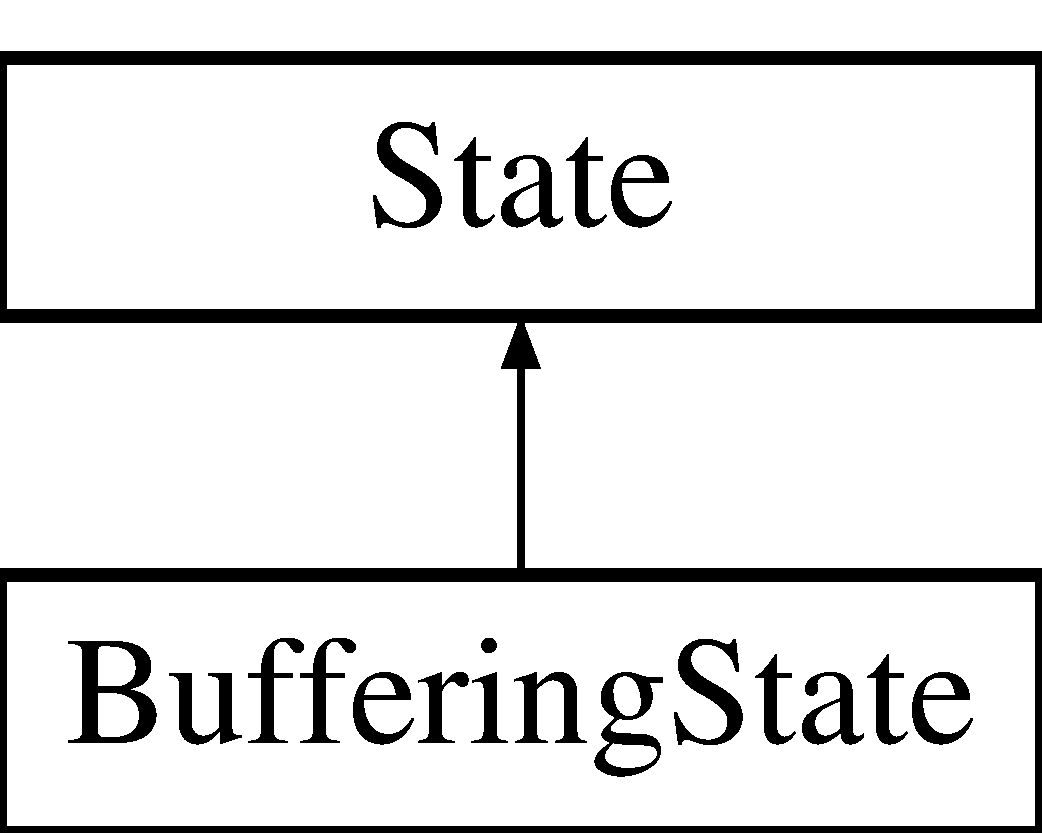
\includegraphics[height=2.000000cm]{classBufferingState}
\end{center}
\end{figure}
\subsection*{Public Member Functions}
\begin{DoxyCompactItemize}
\item 
\hypertarget{classBufferingState_ac17a03512a9faf5f72c85d3a62c18b48}{void {\bfseries setup\-D\-A\-G} (const \hyperlink{structTemplates}{Templates} \&templates)}\label{classBufferingState_ac17a03512a9faf5f72c85d3a62c18b48}

\item 
\hypertarget{classBufferingState_aebc85270708bf8801e76be66c92ea797}{void {\bfseries run} ()}\label{classBufferingState_aebc85270708bf8801e76be66c92ea797}

\item 
\hypertarget{classBufferingState_a03e1dafbc5324854cc8213214ffe6230}{void {\bfseries set\-Source} ()}\label{classBufferingState_a03e1dafbc5324854cc8213214ffe6230}

\end{DoxyCompactItemize}
\subsection*{Public Attributes}
\begin{DoxyCompactItemize}
\item 
\hypertarget{classBufferingState_a82786bc89a2076e2d451c0a94aacb2fb}{\hyperlink{classBufferingDAG__generic}{Buffering\-D\-A\-G\-\_\-generic} {\bfseries buffering\-Graph}}\label{classBufferingState_a82786bc89a2076e2d451c0a94aacb2fb}

\end{DoxyCompactItemize}
\subsection*{Friends}
\begin{DoxyCompactItemize}
\item 
\hypertarget{classBufferingState_ae434ad700893dfcec0c63fdb5a1b7d54}{class {\bfseries T\-E\-S\-T\-\_\-\-Buffering\-State}}\label{classBufferingState_ae434ad700893dfcec0c63fdb5a1b7d54}

\end{DoxyCompactItemize}
\subsection*{Additional Inherited Members}


The documentation for this class was generated from the following files\-:\begin{DoxyCompactItemize}
\item 
/home/rameez/\-Master/\-T\-Ue\-Lane\-Tracker/\-T\-Ue\-L\-D\-T/include/Buffering\-State.\-h\item 
/home/rameez/\-Master/\-T\-Ue\-Lane\-Tracker/\-T\-Ue\-L\-D\-T/Buffering\-State.\-cpp\end{DoxyCompactItemize}

\hypertarget{structBufferPool}{\section{Buffer\-Pool Struct Reference}
\label{structBufferPool}\index{Buffer\-Pool@{Buffer\-Pool}}
}
\subsection*{Public Member Functions}
\begin{DoxyCompactItemize}
\item 
\hypertarget{structBufferPool_a308f8fe879033bfed29a5aa9878e9bf4}{{\bfseries Buffer\-Pool} (const int R\-E\-S\-\_\-\-V, const int R\-E\-S\-\_\-\-H)}\label{structBufferPool_a308f8fe879033bfed29a5aa9878e9bf4}

\end{DoxyCompactItemize}
\subsection*{Public Attributes}
\begin{DoxyCompactItemize}
\item 
\hypertarget{structBufferPool_ae49e6984dda0b1968e6dd9ded3539453}{std\-::array$<$ Mat, State\-::s\-Nb\-Buffer $>$ {\bfseries Probability}}\label{structBufferPool_ae49e6984dda0b1968e6dd9ded3539453}

\item 
\hypertarget{structBufferPool_a30aaffee46f5a4121b349615488bbe9b}{std\-::array$<$ Mat, State\-::s\-Nb\-Buffer $>$ {\bfseries Gradient\-Tangent}}\label{structBufferPool_a30aaffee46f5a4121b349615488bbe9b}

\end{DoxyCompactItemize}


The documentation for this struct was generated from the following file\-:\begin{DoxyCompactItemize}
\item 
/home/rameez/\-Master/\-T\-Ue\-Lane\-Tracker/\-T\-Ue\-L\-D\-T/include/State.\-h\end{DoxyCompactItemize}

\hypertarget{structCamera}{\section{Camera Struct Reference}
\label{structCamera}\index{Camera@{Camera}}
}
\subsection*{Public Attributes}
\begin{DoxyCompactItemize}
\item 
\hypertarget{structCamera_a45708ab1e843379311fd526bb4a714ee}{const Vector2i {\bfseries R\-E\-S\-\_\-\-V\-H}}\label{structCamera_a45708ab1e843379311fd526bb4a714ee}

\item 
\hypertarget{structCamera_a67776a0fb49593b5e52656ed50abe927}{const Vector2i {\bfseries F\-R\-A\-M\-E\-\_\-\-C\-E\-N\-T\-E\-R}}\label{structCamera_a67776a0fb49593b5e52656ed50abe927}

\item 
\hypertarget{structCamera_a09007a033b3e3a1788f6a768f86727ca}{const Vector2f {\bfseries F\-O\-V}}\label{structCamera_a09007a033b3e3a1788f6a768f86727ca}

\item 
\hypertarget{structCamera_ac7e16f6d0f00640b6e6b0e62f9063a9c}{const float {\bfseries H\-E\-I\-G\-H\-T}}\label{structCamera_ac7e16f6d0f00640b6e6b0e62f9063a9c}

\item 
\hypertarget{structCamera_a0c8650cb21e0055fffb14de3a9d0edb3}{const double {\bfseries F\-O\-C\-A\-L\-\_\-\-L\-E\-N\-G\-T\-H}}\label{structCamera_a0c8650cb21e0055fffb14de3a9d0edb3}

\item 
\hypertarget{structCamera_acf6a96f2ca16847f10d5df42275a99ea}{const double {\bfseries C\-M\-\_\-\-T\-O\-\_\-\-P\-I\-X\-E\-L}}\label{structCamera_acf6a96f2ca16847f10d5df42275a99ea}

\end{DoxyCompactItemize}


The documentation for this struct was generated from the following file\-:\begin{DoxyCompactItemize}
\item 
/home/rameez/\-Master/\-T\-Ue\-Lane\-Tracker/\-T\-Ue\-L\-D\-T/include/Camera.\-h\end{DoxyCompactItemize}

\hypertarget{structCar}{\section{Car Struct Reference}
\label{structCar}\index{Car@{Car}}
}
\subsection*{Public Attributes}
\begin{DoxyCompactItemize}
\item 
\hypertarget{structCar_ab939dc98da9e2bcdc07763489903236e}{int {\bfseries Car\-Width\-\_\-cm}}\label{structCar_ab939dc98da9e2bcdc07763489903236e}

\end{DoxyCompactItemize}


The documentation for this struct was generated from the following file\-:\begin{DoxyCompactItemize}
\item 
/home/rameez/\-Master/\-T\-Ue\-Lane\-Tracker/\-T\-Ue\-L\-D\-T/include/Car.\-h\end{DoxyCompactItemize}

\hypertarget{classInitState}{\section{Init\-State Class Reference}
\label{classInitState}\index{Init\-State@{Init\-State}}
}
Inheritance diagram for Init\-State\-:\begin{figure}[H]
\begin{center}
\leavevmode
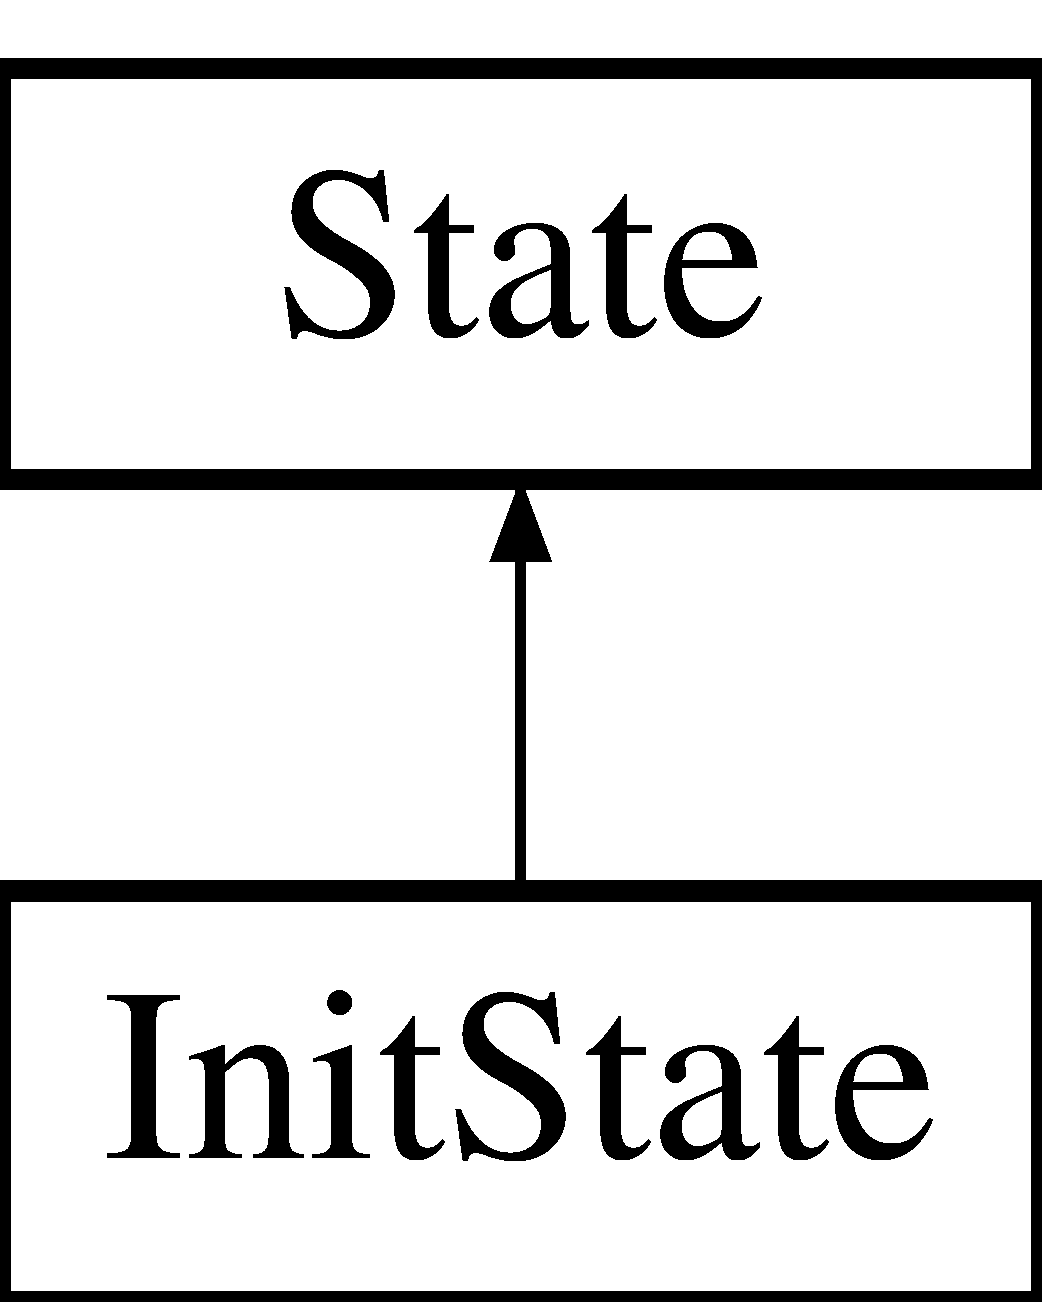
\includegraphics[height=2.000000cm]{classInitState}
\end{center}
\end{figure}
\subsection*{Public Member Functions}
\begin{DoxyCompactItemize}
\item 
\hypertarget{classInitState_a66440894e367dca8890e64a12e013d46}{unique\-\_\-ptr$<$ \hyperlink{classLaneFilter}{Lane\-Filter} $>$ {\bfseries create\-Lane\-Filter} ()}\label{classInitState_a66440894e367dca8890e64a12e013d46}

\item 
\hypertarget{classInitState_af6fb8aac76c287ba445c330b4ba96d17}{unique\-\_\-ptr$<$ \hyperlink{classVanishingPtFilter}{Vanishing\-Pt\-Filter} $>$ {\bfseries create\-Vanishing\-Pt\-Filter} ()}\label{classInitState_af6fb8aac76c287ba445c330b4ba96d17}

\item 
\hypertarget{classInitState_a4c85c3a5f03cc1591762985272ac4544}{unique\-\_\-ptr$<$ \hyperlink{structTemplates}{Templates} $>$ {\bfseries create\-Templates} ()}\label{classInitState_a4c85c3a5f03cc1591762985272ac4544}

\end{DoxyCompactItemize}
\subsection*{Additional Inherited Members}


The documentation for this class was generated from the following files\-:\begin{DoxyCompactItemize}
\item 
/home/rameez/\-Master/\-T\-Ue\-Lane\-Tracker/\-T\-Ue\-L\-D\-T/include/Init\-State.\-h\item 
/home/rameez/\-Master/\-T\-Ue\-Lane\-Tracker/\-T\-Ue\-L\-D\-T/Init\-State.\-cpp\end{DoxyCompactItemize}

\hypertarget{classLaneFilter}{\section{Lane\-Filter Class Reference}
\label{classLaneFilter}\index{Lane\-Filter@{Lane\-Filter}}
}
\subsection*{Public Member Functions}
\begin{DoxyCompactItemize}
\item 
\hypertarget{classLaneFilter_a05e9cf021b1020079d98b61278d78fe2}{{\bfseries Lane\-Filter} (const \hyperlink{structLaneParameters}{Lane\-Parameters} \&L\-A\-N\-E, const \hyperlink{structCamera}{Camera} \&C\-A\-M\-E\-R\-A)}\label{classLaneFilter_a05e9cf021b1020079d98b61278d78fe2}

\end{DoxyCompactItemize}
\subsection*{Public Attributes}
\begin{DoxyCompactItemize}
\item 
\hypertarget{classLaneFilter_ab71c393caf2edf8518576757c5c5c60a}{const int {\bfseries S\-T\-E\-P}}\label{classLaneFilter_ab71c393caf2edf8518576757c5c5c60a}

\item 
\hypertarget{classLaneFilter_a2193e82063749e9aff6f9487d57aaad7}{const int {\bfseries m\-B\-I\-N\-\_\-\-M\-A\-X}}\label{classLaneFilter_a2193e82063749e9aff6f9487d57aaad7}

\item 
\hypertarget{classLaneFilter_a318e84ea645f716c0a66ef83175e8556}{const int {\bfseries m\-Nb\-\_\-\-H\-I\-S\-T\-O\-G\-R\-A\-M\-\_\-\-B\-I\-N\-S}}\label{classLaneFilter_a318e84ea645f716c0a66ef83175e8556}

\item 
\hypertarget{classLaneFilter_a020236f8bcee6881d72a235c111c677f}{const int {\bfseries m\-Nb\-\_\-\-O\-F\-F\-S\-E\-T\-\_\-\-B\-I\-N\-S}}\label{classLaneFilter_a020236f8bcee6881d72a235c111c677f}

\item 
\hypertarget{classLaneFilter_a2dff037db82119c2372d49b5d79ca44e}{const int {\bfseries O\-F\-F\-S\-E\-T\-\_\-\-V}}\label{classLaneFilter_a2dff037db82119c2372d49b5d79ca44e}

\item 
\hypertarget{classLaneFilter_a96434ede64ca9b358416546069ce24b0}{const Vector\-Xi {\bfseries H\-I\-S\-T\-O\-G\-R\-A\-M\-\_\-\-B\-I\-N\-S}}\label{classLaneFilter_a96434ede64ca9b358416546069ce24b0}

\item 
\hypertarget{classLaneFilter_a0cbecdb0c17690f3479ae7bb7a1ed956}{const Vector\-Xi {\bfseries O\-F\-F\-S\-E\-T\-\_\-\-B\-I\-N\-S}}\label{classLaneFilter_a0cbecdb0c17690f3479ae7bb7a1ed956}

\item 
\hypertarget{classLaneFilter_a886dd2f41ef951a1f93227c8ee0b2120}{Mat {\bfseries prior}}\label{classLaneFilter_a886dd2f41ef951a1f93227c8ee0b2120}

\item 
\hypertarget{classLaneFilter_aedbcc4bc3e482a29cdf0ed919d5e0a76}{Mat {\bfseries filter}}\label{classLaneFilter_aedbcc4bc3e482a29cdf0ed919d5e0a76}

\item 
\hypertarget{classLaneFilter_a85aba364e4e6b75313ba9cd450c97fec}{std\-::vector$<$ \hyperlink{structBaseHistogramModel}{Base\-Histogram\-Model} $>$ {\bfseries base\-Histogram\-Models}}\label{classLaneFilter_a85aba364e4e6b75313ba9cd450c97fec}

\end{DoxyCompactItemize}


The documentation for this class was generated from the following files\-:\begin{DoxyCompactItemize}
\item 
/home/rameez/\-Master/\-T\-Ue\-Lane\-Tracker/\-T\-Ue\-L\-D\-T/include/Lane\-Filter.\-h\item 
/home/rameez/\-Master/\-T\-Ue\-Lane\-Tracker/\-T\-Ue\-L\-D\-T/Lane\-Filter.\-cpp\end{DoxyCompactItemize}

\hypertarget{structLaneMembership}{\section{Lane\-Membership Struct Reference}
\label{structLaneMembership}\index{Lane\-Membership@{Lane\-Membership}}
}
\subsection*{Public Attributes}
\begin{DoxyCompactItemize}
\item 
\hypertarget{structLaneMembership_aaafc93ecaca63ffb997f76bb37509e0e}{const uint8\-\_\-t {\bfseries T\-I\-P\-P\-I\-N\-G\-\_\-\-P\-O\-I\-N\-T\-\_\-\-G\-R\-A\-Y}}\label{structLaneMembership_aaafc93ecaca63ffb997f76bb37509e0e}

\item 
\hypertarget{structLaneMembership_a85f42f0e11a66b8e1bf92b196f7b75f2}{const uint8\-\_\-t {\bfseries T\-I\-P\-P\-I\-N\-G\-\_\-\-P\-O\-I\-N\-T\-\_\-\-G\-R\-A\-D\-\_\-\-Mag}}\label{structLaneMembership_a85f42f0e11a66b8e1bf92b196f7b75f2}

\item 
\hypertarget{structLaneMembership_aff8a106dd684a05f84493c60cc1bbbda}{const float {\bfseries W\-I\-D\-T\-H\-\_\-\-D\-I\-F\-F\-\_\-\-N\-O\-R\-M\-A}}\label{structLaneMembership_aff8a106dd684a05f84493c60cc1bbbda}

\item 
\hypertarget{structLaneMembership_a7f5ee55eafd81eb6fcbe68e1751f150e}{const float {\bfseries W\-I\-D\-T\-H\-\_\-\-D\-I\-F\-F\-\_\-\-N\-O\-M\-I\-N}}\label{structLaneMembership_a7f5ee55eafd81eb6fcbe68e1751f150e}

\item 
\hypertarget{structLaneMembership_a99a4cc20750e48c300ca6912654da175}{const float {\bfseries N\-E\-G\-\_\-\-B\-O\-U\-N\-D\-A\-R\-Y\-\_\-\-N\-O\-R\-M\-A}}\label{structLaneMembership_a99a4cc20750e48c300ca6912654da175}

\item 
\hypertarget{structLaneMembership_ac21253cf08f15cf05ff5be79fdf28eb6}{const float {\bfseries N\-E\-G\-\_\-\-B\-O\-U\-N\-D\-A\-R\-Y\-\_\-\-N\-O\-M\-I\-N}}\label{structLaneMembership_ac21253cf08f15cf05ff5be79fdf28eb6}

\end{DoxyCompactItemize}


The documentation for this struct was generated from the following file\-:\begin{DoxyCompactItemize}
\item 
/home/rameez/\-Master/\-T\-Ue\-Lane\-Tracker/\-T\-Ue\-L\-D\-T/include/Lane.\-h\end{DoxyCompactItemize}

\hypertarget{structLaneModel}{\section{Lane\-Model Struct Reference}
\label{structLaneModel}\index{Lane\-Model@{Lane\-Model}}
}
\subsection*{Public Attributes}
\begin{DoxyCompactItemize}
\item 
\hypertarget{structLaneModel_a93d8b45a688c5bd1829f8206dbdf3442}{int {\bfseries left\-Offset}}\label{structLaneModel_a93d8b45a688c5bd1829f8206dbdf3442}

\item 
\hypertarget{structLaneModel_aeb4b4fee6ff618758ce9f5460034a92c}{int {\bfseries right\-Offset}}\label{structLaneModel_aeb4b4fee6ff618758ce9f5460034a92c}

\item 
\hypertarget{structLaneModel_a6de5cb6e6d6677fee8b8e04e1b47964d}{int {\bfseries center\-Lane}}\label{structLaneModel_a6de5cb6e6d6677fee8b8e04e1b47964d}

\item 
\hypertarget{structLaneModel_ae2c26385b345477a2c9bb0eac120efb9}{int {\bfseries confidence\-Left}}\label{structLaneModel_ae2c26385b345477a2c9bb0eac120efb9}

\item 
\hypertarget{structLaneModel_a5faed89e31aa1883f1632f39050081e4}{int {\bfseries confidence\-Right}}\label{structLaneModel_a5faed89e31aa1883f1632f39050081e4}

\item 
\hypertarget{structLaneModel_a4e465e5eb215ef2040a93b0c6e253959}{float {\bfseries lane\-Width\-\_\-cm}}\label{structLaneModel_a4e465e5eb215ef2040a93b0c6e253959}

\end{DoxyCompactItemize}


The documentation for this struct was generated from the following file\-:\begin{DoxyCompactItemize}
\item 
/home/rameez/\-Master/\-T\-Ue\-Lane\-Tracker/\-T\-Ue\-L\-D\-T/include/Lane.\-h\end{DoxyCompactItemize}

\hypertarget{structLaneParameters}{\section{Lane\-Parameters Struct Reference}
\label{structLaneParameters}\index{Lane\-Parameters@{Lane\-Parameters}}
}
\subsection*{Public Attributes}
\begin{DoxyCompactItemize}
\item 
\hypertarget{structLaneParameters_a4e57482888c8554c90892a291b1446a3}{const float {\bfseries A\-V\-G\-\_\-\-W\-I\-D\-T\-H}}\label{structLaneParameters_a4e57482888c8554c90892a291b1446a3}

\item 
\hypertarget{structLaneParameters_af035398d1945296f262ffb74036ad7f6}{const float {\bfseries S\-T\-D\-\_\-\-W\-I\-D\-T\-H}}\label{structLaneParameters_af035398d1945296f262ffb74036ad7f6}

\item 
\hypertarget{structLaneParameters_a20835672f0de66ee93c247dececcf717}{const float {\bfseries M\-I\-N\-\_\-\-W\-I\-D\-T\-H}}\label{structLaneParameters_a20835672f0de66ee93c247dececcf717}

\item 
\hypertarget{structLaneParameters_a21e893076edf22dc4a71e265761a928f}{const float {\bfseries M\-A\-X\-\_\-\-W\-I\-D\-T\-H}}\label{structLaneParameters_a21e893076edf22dc4a71e265761a928f}

\end{DoxyCompactItemize}


The documentation for this struct was generated from the following file\-:\begin{DoxyCompactItemize}
\item 
/home/rameez/\-Master/\-T\-Ue\-Lane\-Tracker/\-T\-Ue\-L\-D\-T/include/Lane.\-h\end{DoxyCompactItemize}

\hypertarget{structPurviewHistogramModel}{\section{Purview\-Histogram\-Model Struct Reference}
\label{structPurviewHistogramModel}\index{Purview\-Histogram\-Model@{Purview\-Histogram\-Model}}
}
\subsection*{Public Attributes}
\begin{DoxyCompactItemize}
\item 
\hypertarget{structPurviewHistogramModel_a2b87493315b13a8b1c5efb9982a2535d}{int {\bfseries bin\-I\-D\-\_\-left\-Boundary}}\label{structPurviewHistogramModel_a2b87493315b13a8b1c5efb9982a2535d}

\item 
\hypertarget{structPurviewHistogramModel_a317eee8ab993e87f6c8d9eaba87ccdef}{int {\bfseries bin\-I\-D\-\_\-right\-Boundary}}\label{structPurviewHistogramModel_a317eee8ab993e87f6c8d9eaba87ccdef}

\item 
\hypertarget{structPurviewHistogramModel_a17410303ad623ea94d7434c8dd04c27c}{int {\bfseries bin\-I\-D\-\_\-\-Neg\-Boundary\-Left}}\label{structPurviewHistogramModel_a17410303ad623ea94d7434c8dd04c27c}

\item 
\hypertarget{structPurviewHistogramModel_ab25fa5ab504e80a8e35a7a21e446d681}{int {\bfseries bin\-I\-D\-\_\-\-Neg\-Boundary\-Right}}\label{structPurviewHistogramModel_ab25fa5ab504e80a8e35a7a21e446d681}

\item 
\hypertarget{structPurviewHistogramModel_a56acc2f5244eab4fe047026d7139bd1e}{int {\bfseries nb\-Non\-Boundary\-Bins\-Left}}\label{structPurviewHistogramModel_a56acc2f5244eab4fe047026d7139bd1e}

\item 
\hypertarget{structPurviewHistogramModel_a4bd03aece0c7ee41ac9aeed7046b8c01}{int {\bfseries nb\-Non\-Boundary\-Bins\-Right}}\label{structPurviewHistogramModel_a4bd03aece0c7ee41ac9aeed7046b8c01}

\end{DoxyCompactItemize}


The documentation for this struct was generated from the following file\-:\begin{DoxyCompactItemize}
\item 
/home/rameez/\-Master/\-T\-Ue\-Lane\-Tracker/\-T\-Ue\-L\-D\-T/include/Vanishing\-Pt\-Filter.\-h\end{DoxyCompactItemize}

\hypertarget{classState}{\section{State Class Reference}
\label{classState}\index{State@{State}}
}
Inheritance diagram for State\-:\begin{figure}[H]
\begin{center}
\leavevmode
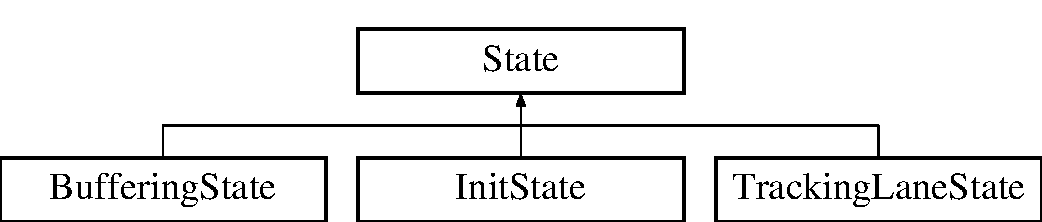
\includegraphics[height=2.000000cm]{classState}
\end{center}
\end{figure}
\subsection*{Public Member Functions}
\begin{DoxyCompactItemize}
\item 
\hypertarget{classState_ad499053c72a0b21c5c9e50456e8f01da}{void {\bfseries conclude} ()}\label{classState_ad499053c72a0b21c5c9e50456e8f01da}

\end{DoxyCompactItemize}
\subsection*{Public Attributes}
\begin{DoxyCompactItemize}
\item 
\hypertarget{classState_acc98ede8633918c2077fbc204b4b6bad}{int64\-\_\-t {\bfseries State\-Counter}}\label{classState_acc98ede8633918c2077fbc204b4b6bad}

\item 
\hypertarget{classState_a62a87cbab86fe461f6a66c98a98abac0}{State\-Status {\bfseries current\-Status}}\label{classState_a62a87cbab86fe461f6a66c98a98abac0}

\end{DoxyCompactItemize}
\subsection*{Static Public Attributes}
\begin{DoxyCompactItemize}
\item 
\hypertarget{classState_a753c5c7247802fe071e3d8d73e5733f7}{static const int {\bfseries s\-Nb\-Buffer} =5}\label{classState_a753c5c7247802fe071e3d8d73e5733f7}

\end{DoxyCompactItemize}


The documentation for this class was generated from the following files\-:\begin{DoxyCompactItemize}
\item 
/home/rameez/\-Master/\-T\-Ue\-Lane\-Tracker/\-T\-Ue\-L\-D\-T/include/State.\-h\item 
/home/rameez/\-Master/\-T\-Ue\-Lane\-Tracker/\-T\-Ue\-L\-D\-T/State.\-cpp\end{DoxyCompactItemize}

\hypertarget{classStateMachine}{\section{State\-Machine Class Reference}
\label{classStateMachine}\index{State\-Machine@{State\-Machine}}
}
\subsection*{Public Member Functions}
\begin{DoxyCompactItemize}
\item 
\hypertarget{classStateMachine_a3dd8562cc7ad040b2392db8771165c7e}{int {\bfseries spin} (shared\-\_\-ptr$<$ Sig\-Init $>$)}\label{classStateMachine_a3dd8562cc7ad040b2392db8771165c7e}

\end{DoxyCompactItemize}


The documentation for this class was generated from the following files\-:\begin{DoxyCompactItemize}
\item 
/home/rameez/\-Master/\-T\-Ue\-Lane\-Tracker/\-T\-Ue\-L\-D\-T/include/State\-Machine.\-h\item 
/home/rameez/\-Master/\-T\-Ue\-Lane\-Tracker/\-T\-Ue\-L\-D\-T/State\-Machine.\-cpp\end{DoxyCompactItemize}

\hypertarget{structTemplates}{\section{Templates Struct Reference}
\label{structTemplates}\index{Templates@{Templates}}
}
\subsection*{Public Member Functions}
\begin{DoxyCompactItemize}
\item 
\hypertarget{structTemplates_aeacfc38018e21a2df493336224208531}{{\bfseries Templates} (const int R\-E\-S\-\_\-\-V, const int R\-E\-S\-\_\-\-H, const int V\-P\-\_\-\-R\-A\-N\-G\-E\-\_\-\-R\-O\-W\-S)}\label{structTemplates_aeacfc38018e21a2df493336224208531}

\end{DoxyCompactItemize}
\subsection*{Public Attributes}
\begin{DoxyCompactItemize}
\item 
\hypertarget{structTemplates_a180d049978ef6aad917be35df074beb2}{const int {\bfseries M\-A\-R\-G\-I\-N}}\label{structTemplates_a180d049978ef6aad917be35df074beb2}

\item 
\hypertarget{structTemplates_a612f7f272237dad815f4f0f9048dfc5e}{const int {\bfseries V\-P\-\_\-\-R\-A\-N\-G\-E\-\_\-\-V}}\label{structTemplates_a612f7f272237dad815f4f0f9048dfc5e}

\item 
\hypertarget{structTemplates_a3ac851da69759a72b3a63ddf633c884b}{const int {\bfseries S\-P\-A\-N}}\label{structTemplates_a3ac851da69759a72b3a63ddf633c884b}

\item 
\hypertarget{structTemplates_a523f278fb43e933ad253b350af123ad0}{Mat {\bfseries G\-R\-A\-D\-I\-E\-N\-T\-\_\-\-T\-A\-N\-\_\-\-R\-O\-O\-T}}\label{structTemplates_a523f278fb43e933ad253b350af123ad0}

\item 
\hypertarget{structTemplates_aed48eeb4f1fdd5d19ae81db84b69e6a7}{Mat {\bfseries F\-O\-C\-U\-S\-\_\-\-M\-A\-S\-K\-\_\-\-R\-O\-O\-T}}\label{structTemplates_aed48eeb4f1fdd5d19ae81db84b69e6a7}

\item 
\hypertarget{structTemplates_a9b7438fec160d2ecfc8ce4da697e48c3}{Mat {\bfseries D\-E\-P\-T\-H\-\_\-\-M\-A\-P\-\_\-\-R\-O\-O\-T}}\label{structTemplates_a9b7438fec160d2ecfc8ce4da697e48c3}

\item 
\hypertarget{structTemplates_a618ff0f5efcd3580e6141d21ad9fe004}{Mat {\bfseries X\-\_\-\-I\-R\-S}}\label{structTemplates_a618ff0f5efcd3580e6141d21ad9fe004}

\item 
\hypertarget{structTemplates_a7716055d360bc6661b7a20d3ad766504}{Mat {\bfseries Y\-\_\-\-I\-R\-S}}\label{structTemplates_a7716055d360bc6661b7a20d3ad766504}

\end{DoxyCompactItemize}


The documentation for this struct was generated from the following file\-:\begin{DoxyCompactItemize}
\item 
/home/rameez/\-Master/\-T\-Ue\-Lane\-Tracker/\-T\-Ue\-L\-D\-T/include/Templates.\-h\end{DoxyCompactItemize}

\hypertarget{classTrackingLaneDAG__generic}{\section{Tracking\-Lane\-D\-A\-G\-\_\-generic Class Reference}
\label{classTrackingLaneDAG__generic}\index{Tracking\-Lane\-D\-A\-G\-\_\-generic@{Tracking\-Lane\-D\-A\-G\-\_\-generic}}
}
Inheritance diagram for Tracking\-Lane\-D\-A\-G\-\_\-generic\-:\begin{figure}[H]
\begin{center}
\leavevmode
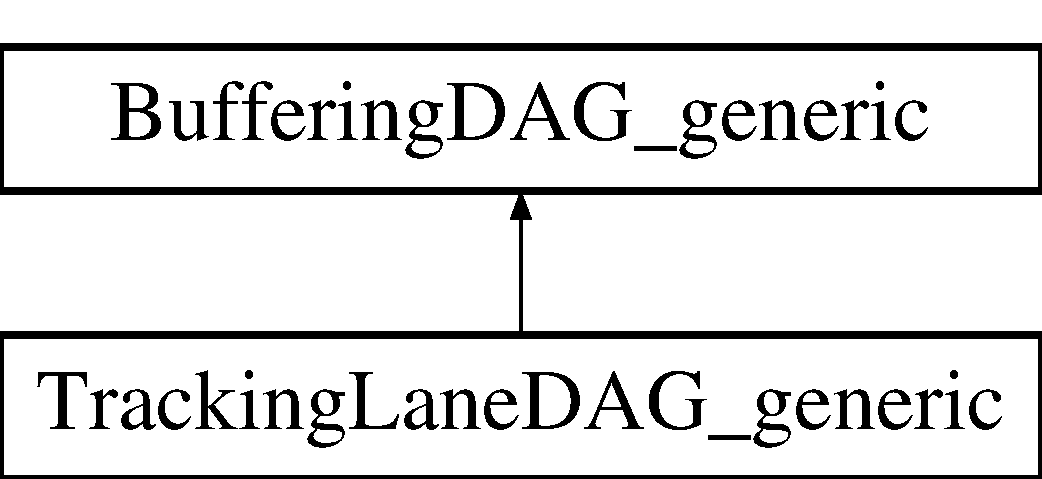
\includegraphics[height=2.000000cm]{classTrackingLaneDAG__generic}
\end{center}
\end{figure}
\subsection*{Public Member Functions}
\begin{DoxyCompactItemize}
\item 
\hypertarget{classTrackingLaneDAG__generic_adb64af801b50375a3f27aaf228d10a09}{{\bfseries Tracking\-Lane\-D\-A\-G\-\_\-generic} (\hyperlink{classBufferingDAG__generic}{Buffering\-D\-A\-G\-\_\-generic} \&\&buffering\-Graph)}\label{classTrackingLaneDAG__generic_adb64af801b50375a3f27aaf228d10a09}

\item 
\hypertarget{classTrackingLaneDAG__generic_a52e21e76e2751170a3a43ce303e3523e}{void {\bfseries auxillary\-Tasks} ()}\label{classTrackingLaneDAG__generic_a52e21e76e2751170a3a43ce303e3523e}

\item 
\hypertarget{classTrackingLaneDAG__generic_a6ae6159ff33fc58e7ee158cabba7cb23}{void {\bfseries extract\-Lanes} ()}\label{classTrackingLaneDAG__generic_a6ae6159ff33fc58e7ee158cabba7cb23}

\item 
\hypertarget{classTrackingLaneDAG__generic_a9ca038fa0421160e4445d6936f986e89}{void {\bfseries extract\-Controller\-Inputs} ()}\label{classTrackingLaneDAG__generic_a9ca038fa0421160e4445d6936f986e89}

\end{DoxyCompactItemize}
\subsection*{Friends}
\begin{DoxyCompactItemize}
\item 
\hypertarget{classTrackingLaneDAG__generic_aac458818b6cd604399e29b1702515238}{class {\bfseries Tracking\-Lane\-State}}\label{classTrackingLaneDAG__generic_aac458818b6cd604399e29b1702515238}

\item 
\hypertarget{classTrackingLaneDAG__generic_a3084c090c58f2a0dcf5e638b19d63653}{class {\bfseries T\-E\-S\-T\-\_\-\-Tracking\-State}}\label{classTrackingLaneDAG__generic_a3084c090c58f2a0dcf5e638b19d63653}

\end{DoxyCompactItemize}
\subsection*{Additional Inherited Members}


The documentation for this class was generated from the following files\-:\begin{DoxyCompactItemize}
\item 
/home/rameez/\-Master/\-T\-Ue\-Lane\-Tracker/\-T\-Ue\-L\-D\-T/include/Tracking\-Lane\-D\-A\-G\-\_\-generic.\-h\item 
/home/rameez/\-Master/\-T\-Ue\-Lane\-Tracker/\-T\-Ue\-L\-D\-T/Tracking\-Lane\-D\-A\-G\-\_\-generic.\-cpp\end{DoxyCompactItemize}

\hypertarget{classTrackingLaneState}{\section{Tracking\-Lane\-State Class Reference}
\label{classTrackingLaneState}\index{Tracking\-Lane\-State@{Tracking\-Lane\-State}}
}
Inheritance diagram for Tracking\-Lane\-State\-:\begin{figure}[H]
\begin{center}
\leavevmode
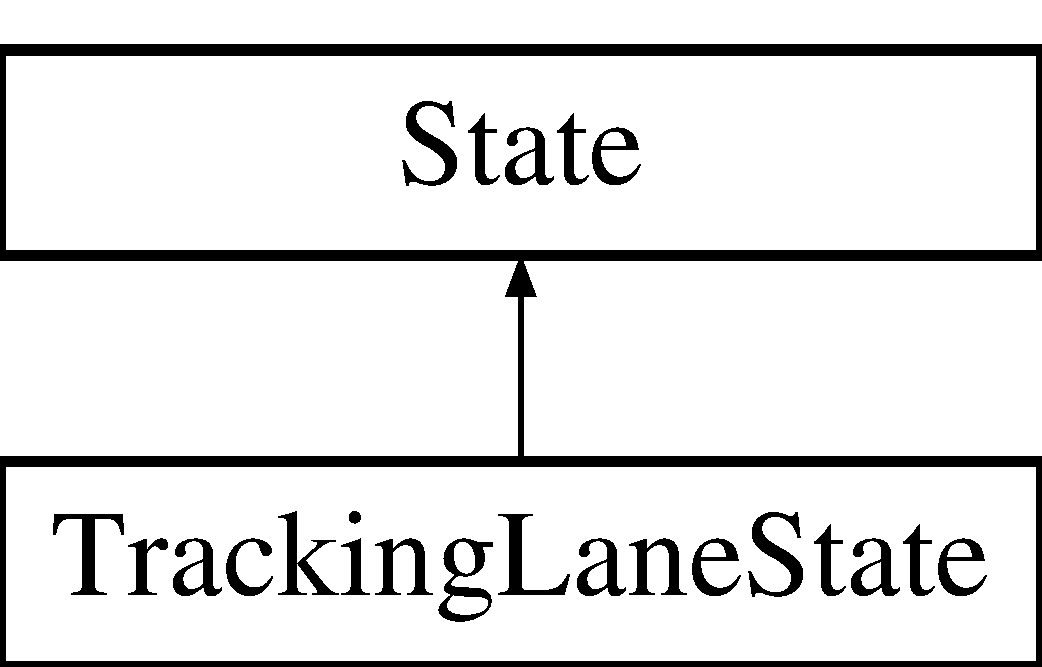
\includegraphics[height=2.000000cm]{classTrackingLaneState}
\end{center}
\end{figure}
\subsection*{Public Member Functions}
\begin{DoxyCompactItemize}
\item 
\hypertarget{classTrackingLaneState_ac57803df98ba03024c29ad864fddea11}{void {\bfseries run} ()}\label{classTrackingLaneState_ac57803df98ba03024c29ad864fddea11}

\item 
\hypertarget{classTrackingLaneState_a5f769fb1982e95791b5735844e5c0aa2}{void {\bfseries setup\-D\-A\-G} (\hyperlink{classLaneFilter}{Lane\-Filter} $\ast$lane\-Filter, \hyperlink{classVanishingPtFilter}{Vanishing\-Pt\-Filter} $\ast$vp\-Filter)}\label{classTrackingLaneState_a5f769fb1982e95791b5735844e5c0aa2}

\item 
\hypertarget{classTrackingLaneState_a77d46118062db8bdc0b114baaaece36e}{{\bfseries Tracking\-Lane\-State} (\hyperlink{classBufferingDAG__generic}{Buffering\-D\-A\-G\-\_\-generic} \&\&buffering\-Graph)}\label{classTrackingLaneState_a77d46118062db8bdc0b114baaaece36e}

\end{DoxyCompactItemize}
\subsection*{Friends}
\begin{DoxyCompactItemize}
\item 
\hypertarget{classTrackingLaneState_a3084c090c58f2a0dcf5e638b19d63653}{class {\bfseries T\-E\-S\-T\-\_\-\-Tracking\-State}}\label{classTrackingLaneState_a3084c090c58f2a0dcf5e638b19d63653}

\end{DoxyCompactItemize}
\subsection*{Additional Inherited Members}


The documentation for this class was generated from the following files\-:\begin{DoxyCompactItemize}
\item 
/home/rameez/\-Master/\-T\-Ue\-Lane\-Tracker/\-T\-Ue\-L\-D\-T/include/Tracking\-Lane\-State.\-h\item 
/home/rameez/\-Master/\-T\-Ue\-Lane\-Tracker/\-T\-Ue\-L\-D\-T/Tracking\-Lane\-State.\-cpp\end{DoxyCompactItemize}

\hypertarget{structVanishingPt}{\section{Vanishing\-Pt Struct Reference}
\label{structVanishingPt}\index{Vanishing\-Pt@{Vanishing\-Pt}}
}
\subsection*{Public Attributes}
\begin{DoxyCompactItemize}
\item 
\hypertarget{structVanishingPt_a6d9909ba6a33313168a95a84c9f8e944}{int {\bfseries V}}\label{structVanishingPt_a6d9909ba6a33313168a95a84c9f8e944}

\item 
\hypertarget{structVanishingPt_abe4867620d0ccf017a4cdab7d7b8d9c1}{int {\bfseries H}}\label{structVanishingPt_abe4867620d0ccf017a4cdab7d7b8d9c1}

\item 
\hypertarget{structVanishingPt_ad996aee9893bacc7ca79ce8da5c7ef23}{int {\bfseries V\-\_\-prev}}\label{structVanishingPt_ad996aee9893bacc7ca79ce8da5c7ef23}

\item 
\hypertarget{structVanishingPt_a83e330bc4a84c5a8cba78838d2eb6bd3}{int {\bfseries H\-\_\-prev}}\label{structVanishingPt_a83e330bc4a84c5a8cba78838d2eb6bd3}

\end{DoxyCompactItemize}


The documentation for this struct was generated from the following file\-:\begin{DoxyCompactItemize}
\item 
/home/rameez/\-Master/\-T\-Ue\-Lane\-Tracker/\-T\-Ue\-L\-D\-T/include/Vanishing\-Pt\-Filter.\-h\end{DoxyCompactItemize}

\hypertarget{classVanishingPtFilter}{\section{Vanishing\-Pt\-Filter Class Reference}
\label{classVanishingPtFilter}\index{Vanishing\-Pt\-Filter@{Vanishing\-Pt\-Filter}}
}
\subsection*{Public Member Functions}
\begin{DoxyCompactItemize}
\item 
\hypertarget{classVanishingPtFilter_a3ecfb92539e41bc01a16e9e71e917e48}{{\bfseries Vanishing\-Pt\-Filter} (const Ref$<$ const Vector\-Xi $>$ \&L\-A\-N\-E\-\_\-\-H\-I\-S\-T\-O\-G\-R\-A\-M\-\_\-\-B\-I\-N\-S, const int \&L\-A\-N\-E\-\_\-\-F\-I\-L\-T\-E\-R\-\_\-\-O\-F\-F\-S\-E\-T\-\_\-\-V)}\label{classVanishingPtFilter_a3ecfb92539e41bc01a16e9e71e917e48}

\end{DoxyCompactItemize}
\subsection*{Public Attributes}
\begin{DoxyCompactItemize}
\item 
\hypertarget{classVanishingPtFilter_a2afd973eb76166b4509d9d632e79a483}{const int {\bfseries V\-P\-\_\-\-R\-A\-N\-G\-E\-\_\-\-V}}\label{classVanishingPtFilter_a2afd973eb76166b4509d9d632e79a483}

\item 
\hypertarget{classVanishingPtFilter_aba7227752de1efa670a59ccfd2517b60}{const int {\bfseries V\-P\-\_\-\-R\-A\-N\-G\-E\-\_\-\-H}}\label{classVanishingPtFilter_aba7227752de1efa670a59ccfd2517b60}

\item 
\hypertarget{classVanishingPtFilter_ac82cb016f56a37fcb1a503e11e22e3c0}{const int {\bfseries m\-Nb\-\_\-\-V\-P\-\_\-\-B\-I\-N\-S\-\_\-\-V}}\label{classVanishingPtFilter_ac82cb016f56a37fcb1a503e11e22e3c0}

\item 
\hypertarget{classVanishingPtFilter_af83d2e2a40ff748dcf9a77864b0bd450}{const int {\bfseries m\-Nb\-\_\-\-V\-P\-\_\-\-B\-I\-N\-S\-\_\-\-H}}\label{classVanishingPtFilter_af83d2e2a40ff748dcf9a77864b0bd450}

\item 
\hypertarget{classVanishingPtFilter_ac4963f559c9751d9e0beb880e107d33a}{const Vector\-Xi {\bfseries V\-P\-\_\-\-B\-I\-N\-S\-\_\-\-V}}\label{classVanishingPtFilter_ac4963f559c9751d9e0beb880e107d33a}

\item 
\hypertarget{classVanishingPtFilter_a3a40af648bfed495a65227f6e22f65e3}{const Vector\-Xi {\bfseries V\-P\-\_\-\-B\-I\-N\-S\-\_\-\-H}}\label{classVanishingPtFilter_a3a40af648bfed495a65227f6e22f65e3}

\item 
\hypertarget{classVanishingPtFilter_a4ad42b4d6a5a2d102748738e6e82b0da}{const int {\bfseries O\-F\-F\-S\-E\-T\-\_\-\-V}}\label{classVanishingPtFilter_a4ad42b4d6a5a2d102748738e6e82b0da}

\item 
\hypertarget{classVanishingPtFilter_a9817529f64ae5a4e8432a4d5ba276133}{const float {\bfseries m\-V\-P\-\_\-\-L\-A\-N\-E\-\_\-\-R\-A\-T\-I\-O}}\label{classVanishingPtFilter_a9817529f64ae5a4e8432a4d5ba276133}

\item 
\hypertarget{classVanishingPtFilter_a063d8af6b02b1f9fdaeaffaeca363f03}{const Vector\-Xi {\bfseries H\-I\-S\-T\-O\-G\-R\-A\-M\-\_\-\-B\-I\-N\-S}}\label{classVanishingPtFilter_a063d8af6b02b1f9fdaeaffaeca363f03}

\item 
\hypertarget{classVanishingPtFilter_a084eec87dd13ebbb5dfb4fdb7429a7bd}{const int {\bfseries S\-T\-E\-P}}\label{classVanishingPtFilter_a084eec87dd13ebbb5dfb4fdb7429a7bd}

\item 
\hypertarget{classVanishingPtFilter_abe37dbf0f29cc77268c7f9a2a1002e20}{Mat {\bfseries prior}}\label{classVanishingPtFilter_abe37dbf0f29cc77268c7f9a2a1002e20}

\item 
\hypertarget{classVanishingPtFilter_a6e143ceb334bb8a17af060d4c5fd7f16}{Mat {\bfseries filter}}\label{classVanishingPtFilter_a6e143ceb334bb8a17af060d4c5fd7f16}

\end{DoxyCompactItemize}


The documentation for this class was generated from the following files\-:\begin{DoxyCompactItemize}
\item 
/home/rameez/\-Master/\-T\-Ue\-Lane\-Tracker/\-T\-Ue\-L\-D\-T/include/Vanishing\-Pt\-Filter.\-h\item 
/home/rameez/\-Master/\-T\-Ue\-Lane\-Tracker/\-T\-Ue\-L\-D\-T/Vanishing\-Pt\-Filter.\-cpp\end{DoxyCompactItemize}

\chapter{File Documentation}
\hypertarget{main_8cpp}{\section{/home/rameez/\-Master/\-T\-Ue\-Lane\-Tracker/\-Lane\-Tracker\-App/main.cpp File Reference}
\label{main_8cpp}\index{/home/rameez/\-Master/\-T\-Ue\-Lane\-Tracker/\-Lane\-Tracker\-App/main.\-cpp@{/home/rameez/\-Master/\-T\-Ue\-Lane\-Tracker/\-Lane\-Tracker\-App/main.\-cpp}}
}
{\ttfamily \#include \char`\"{}opencv2/opencv.\-hpp\char`\"{}}\\*
{\ttfamily \#include \char`\"{}opencv2/highgui/highgui.\-hpp\char`\"{}}\\*
{\ttfamily \#include \char`\"{}State\-Machine.\-h\char`\"{}}\\*
\subsection*{Functions}
\begin{DoxyCompactItemize}
\item 
int \hyperlink{main_8cpp_ae66f6b31b5ad750f1fe042a706a4e3d4}{main} ()
\end{DoxyCompactItemize}


\subsection{Function Documentation}
\hypertarget{main_8cpp_ae66f6b31b5ad750f1fe042a706a4e3d4}{\index{main.\-cpp@{main.\-cpp}!main@{main}}
\index{main@{main}!main.cpp@{main.\-cpp}}
\subsubsection[{main}]{\setlength{\rightskip}{0pt plus 5cm}int main (
\begin{DoxyParamCaption}
{}
\end{DoxyParamCaption}
)}}\label{main_8cpp_ae66f6b31b5ad750f1fe042a706a4e3d4}
This is the entry point of the application.
\begin{DoxyItemize}
\item Sets the path to the input images if flag D\-I\-R\-E\-C\-T\-O\-R\-Y\-\_\-\-I\-N\-P\-U\-T is defined
\item Initialises the sig\-Init handler
\item Creates a state\-Machine and spins it until user issues a quit signal through the sig\-Init handler. 
\end{DoxyItemize}
%--- End generated contents ---

% Index
\newpage
\phantomsection
\addcontentsline{toc}{chapter}{Index}
\printindex

\end{document}
